\chapter{Results}
\label{ch:results}

The results of the experiments conducted in this study are presented in this chapter. The findings are organized according to the research questions outlined in Chapter \ref{ch:intro}. Each section provides a detailed analysis of the results, including relevant figures and tables to support the findings. Detailed analysis of the results will follow in Chapter \ref{ch:discuss}.

\section{Manual Exploration of Dataset}

\begin{figure}[ht]
    \centering
    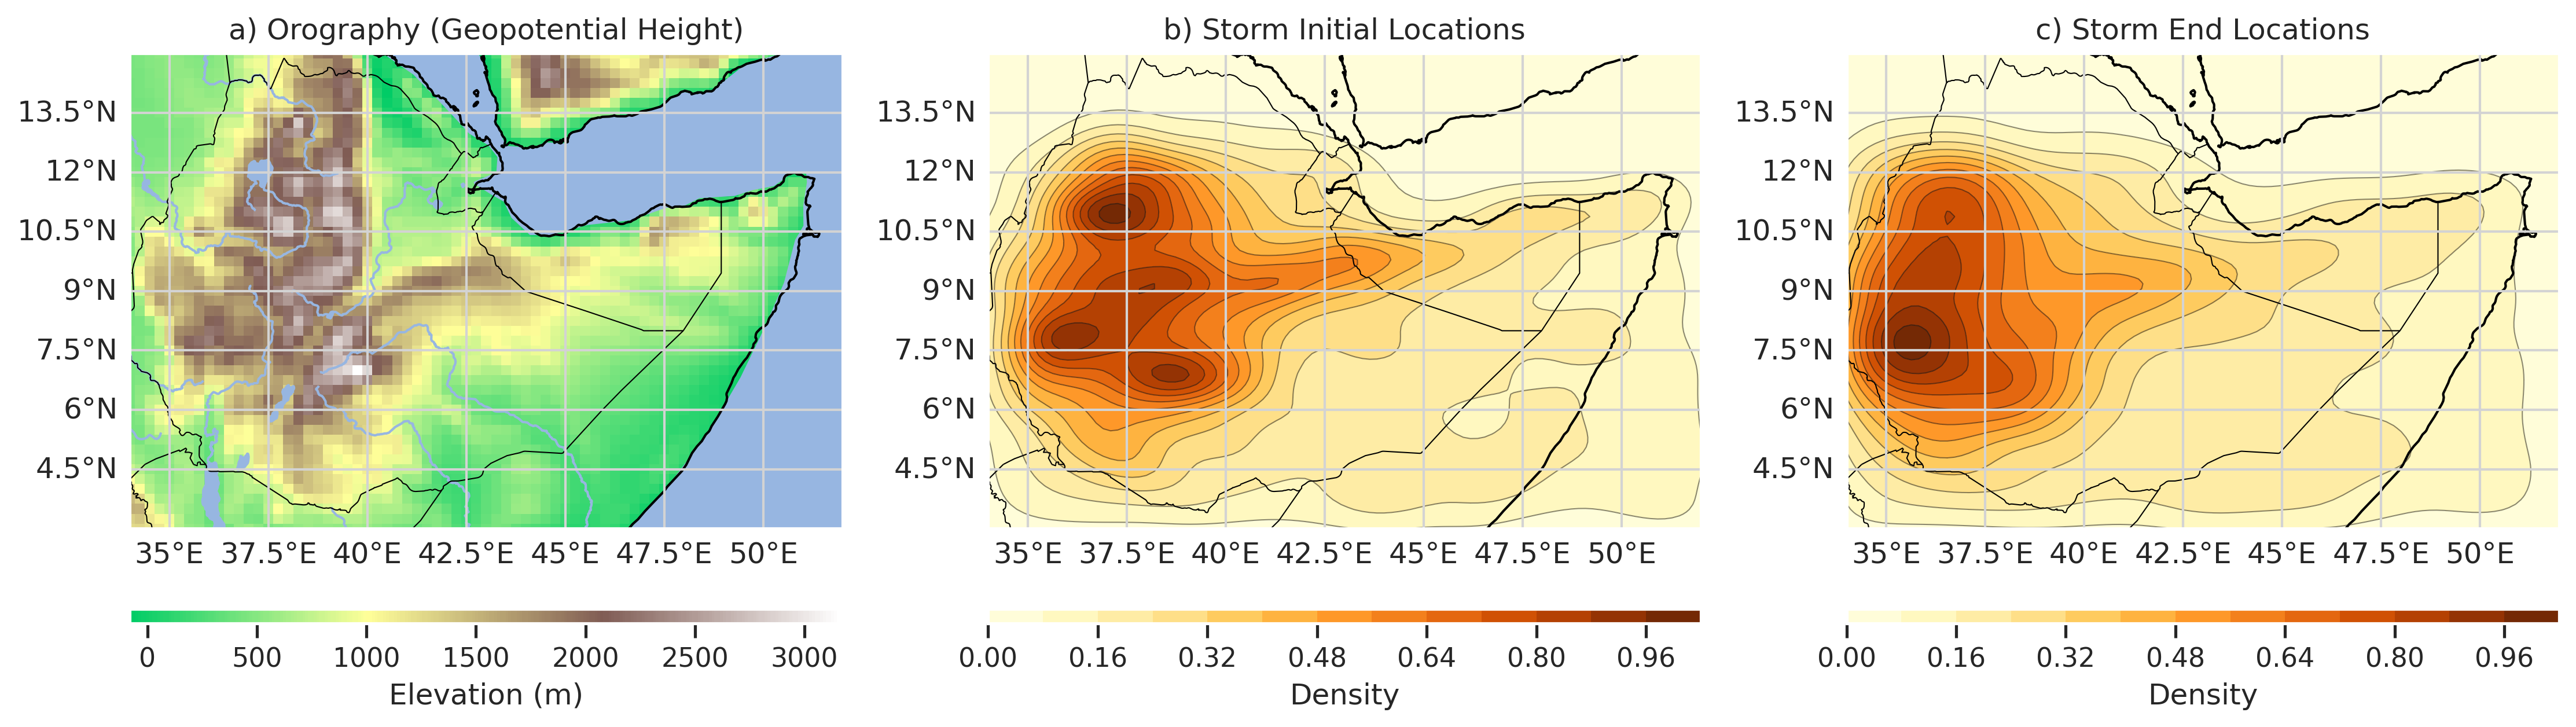
\includegraphics[width=\textwidth]{../figures/generated/exploration/orography_storm_init_end_kde.png}
    \caption{Storm start and end location density. Storms were selected if 1) they last longer than 3 hours to precipitation contributions, and 2) their centroids are located within \degN{3} - \degN{15} and \degE{34} - \degE{52} \citep{Hill2023}. See Chapter \ref{ch:method} for details. Elevation was calculated from \acrshort{era5} geopotential height data.}
    \label{fig:orography_storm_init_end_kde}
\end{figure}

\begin{figure}[ht]
    \centering
    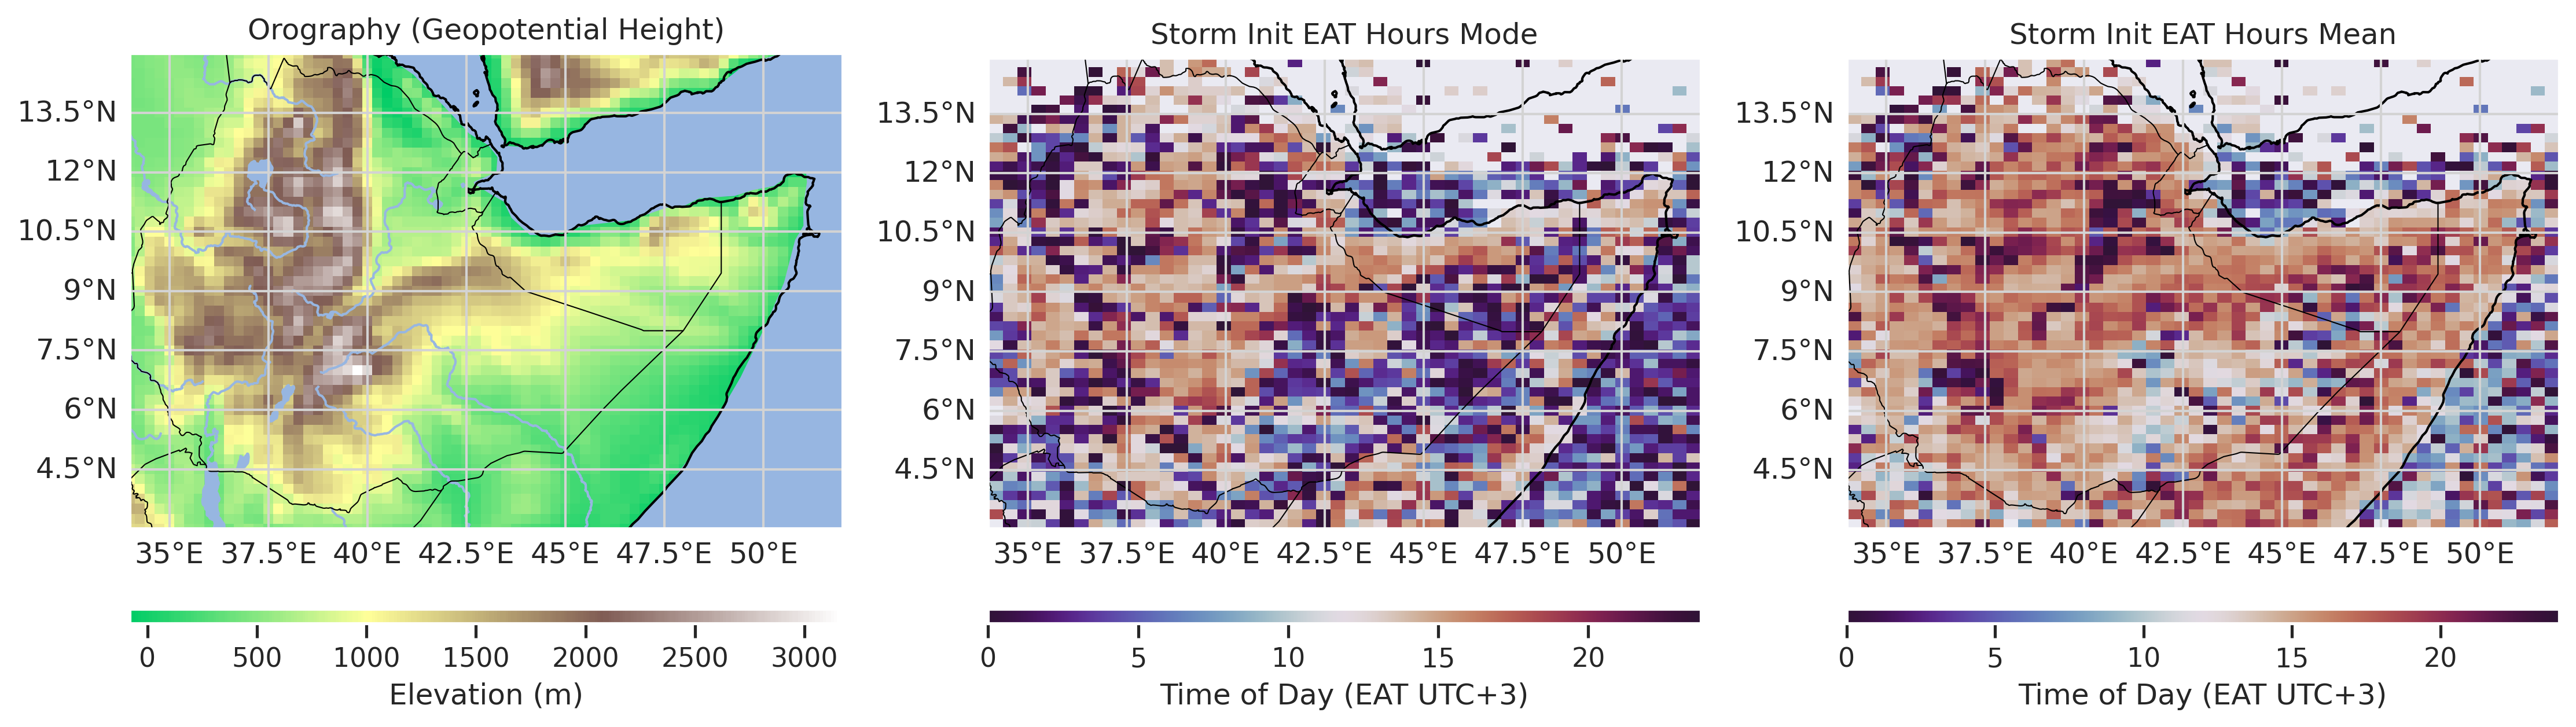
\includegraphics[width=\textwidth]{../figures/generated/exploration/orography_storm_init_eat_hours_mode_mean.png}
    \caption{Storm Genesis Local Time (\acrlong{eat}). Elevation was calculated from \acrshort{era5} geopotential height data.}
    \label{fig:orography_storm_init_eat_hours_mode_mean}
\end{figure}

\section{Experimental Results Overview}

This section provides an overview of the experimental results obtained from the various predictive tasks outlined in the methodology. The results are categorised based on the type of prediction: storm aggregate features and immediate characteristics at an observation. 

\section{Predict Storm Aggregate Features}

These experiments aim to predict the overall characteristics of a storm based on its initial observation.

\subsection{Storm Max Intensity}

Table \ref{tab:storm_max_intensity_results} details the performance metrics for storm max intensity prediction across different experimental setups as specified in the methodology. Note that the target predictand was \texttt{storm\_min\_bt} so lower values indicate stronger storms.

The key observations include: \todo{make a paragraph}
\begin{itemize}
    \item ERA5 features alone perform comparably to all features
    \item Using only the first points results in a substantial drop in performance
\end{itemize}

\begin{table}[ht]
\centering
\caption{Experiment results for storm max intensity prediction}
\label{tab:storm_max_intensity_results}
\begin{tabular}{lccccc}
\hline
\textbf{Experiment} & \multicolumn{2}{c}{\textbf{RMSE}} & \multicolumn{2}{c}{\textbf{Target Std}} & \textbf{Actual vs. Predicted $R^2$} \\
\cline{2-5}
 & \textbf{All} & \textbf{First pts} & \textbf{All} & \textbf{First pts} &  \\
\hline
All              & 2.7610 & 4.4872 & 9.1679 & 8.8540 & 0.9098 \\
\acrshort{era5}             & 2.7503 & 4.1075 & 9.1679 & 8.8540 & 0.9134 \\
All First Points & \multicolumn{2}{c}{7.2265} & \multicolumn{2}{c}{8.9432} & 0.3478 \\
\acrshort{era5} First Points & \multicolumn{2}{c}{7.4673} & \multicolumn{2}{c}{8.9432} & 0.3034 \\
\hline
\end{tabular}
\end{table}

Due to the poor performance of the first points only models, further explainability analysis will focus on the all observations models.

\begin{figure}[h]
    \centering
    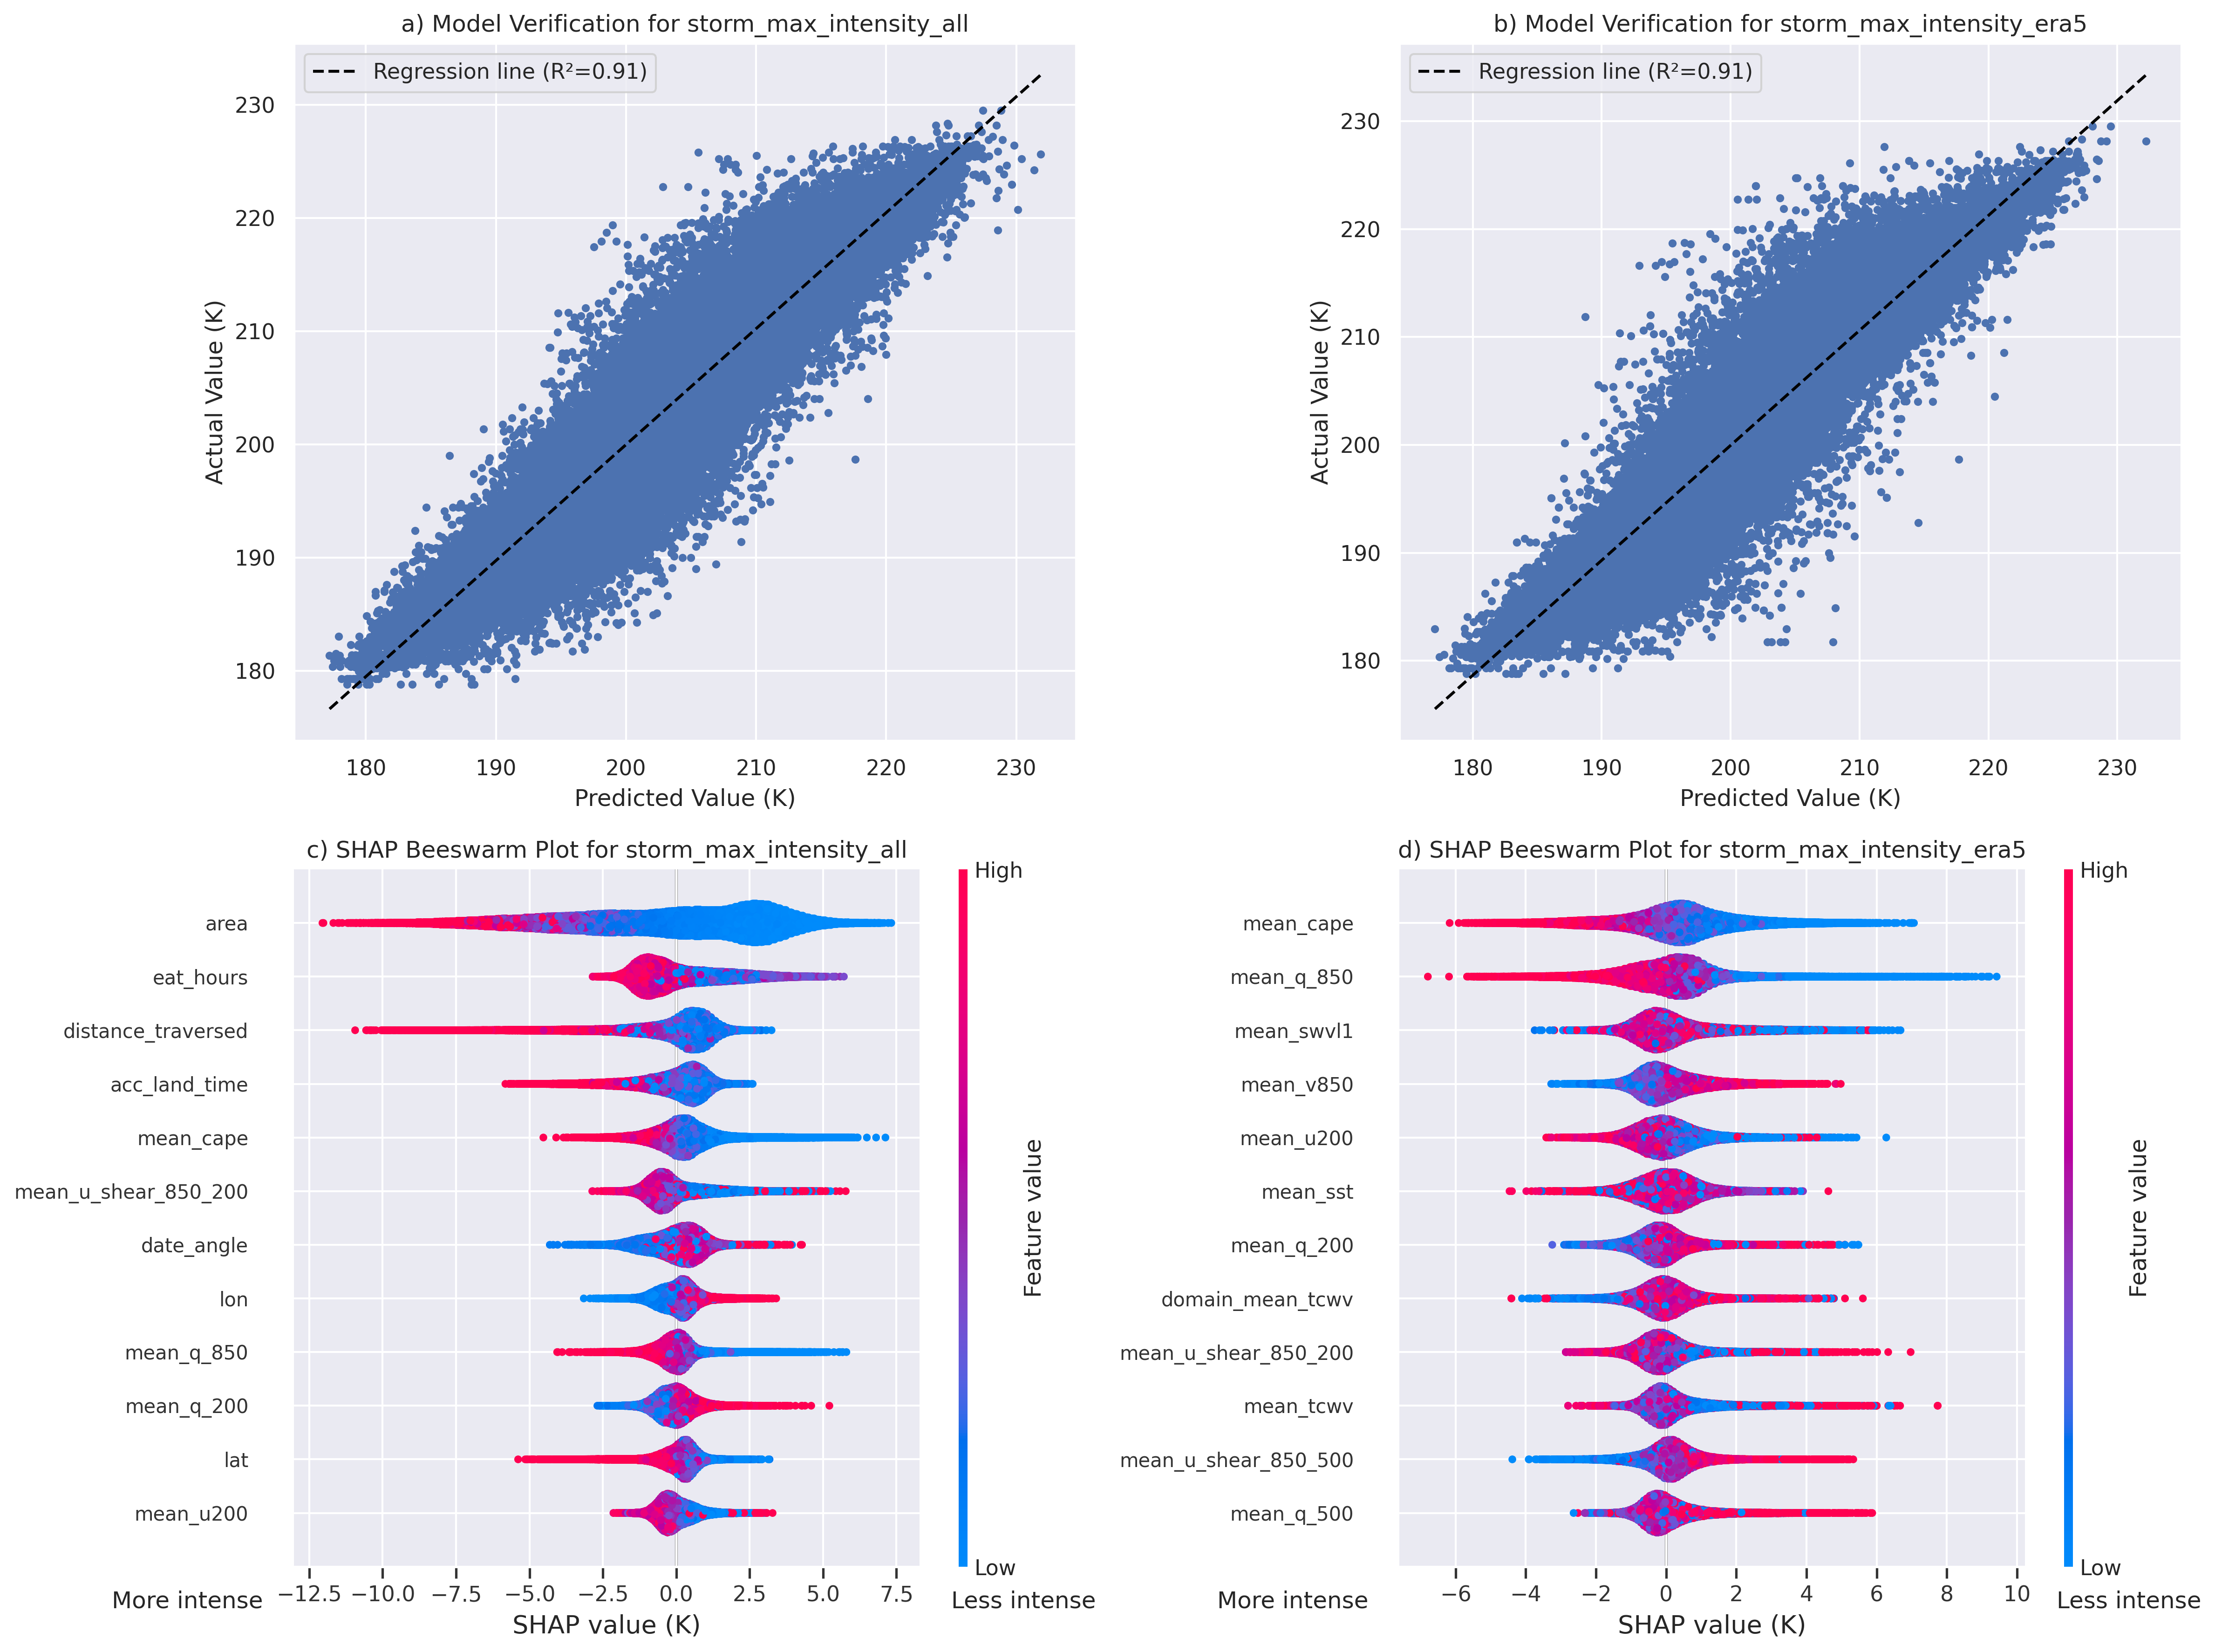
\includegraphics[width=\textwidth]{../figures/generated/experiments/storm_max_intensity/storm_max_intensity_summary.png}
    \caption{Comparison of performance and top features for storm max intensity.}
    \label{fig:storm_max_intensity_summary}
\end{figure}

Figure \ref{fig:storm_max_intensity_summary} presents a detailed comparison of the model performance and the most influential features for predicting storm max intensity using all features versus \acrshort{era5} only.

The key observations include: \todo{make a paragraph}
\begin{itemize}
    \item only one meteorological variable in top 5 for all features model from c)
    \item diurnal cycle is clear with stronger storms developing in late evening from c)
    \item \acrshort{cape} is reliably the most important meteorological factor from c) and d)
\end{itemize}

Particularly notable for these models is that the importance of low-level meridional winds changes with time of day, date, and location. Figure \ref{fig:storm_max_intensity_era5_shap_mean_v850_map_by_month} illustrates this variability over the study region throughout the year. During the summer months, the influence is predominantly positive over the Somali coastal plains and negative over the Ethiopian Highlands, indicating a diminishing effect on storm intensity in the southeast. Conversely, in the winter months, the influence tends to be negative or neutral over the entire domain.

\begin{figure}[h]
    \centering
    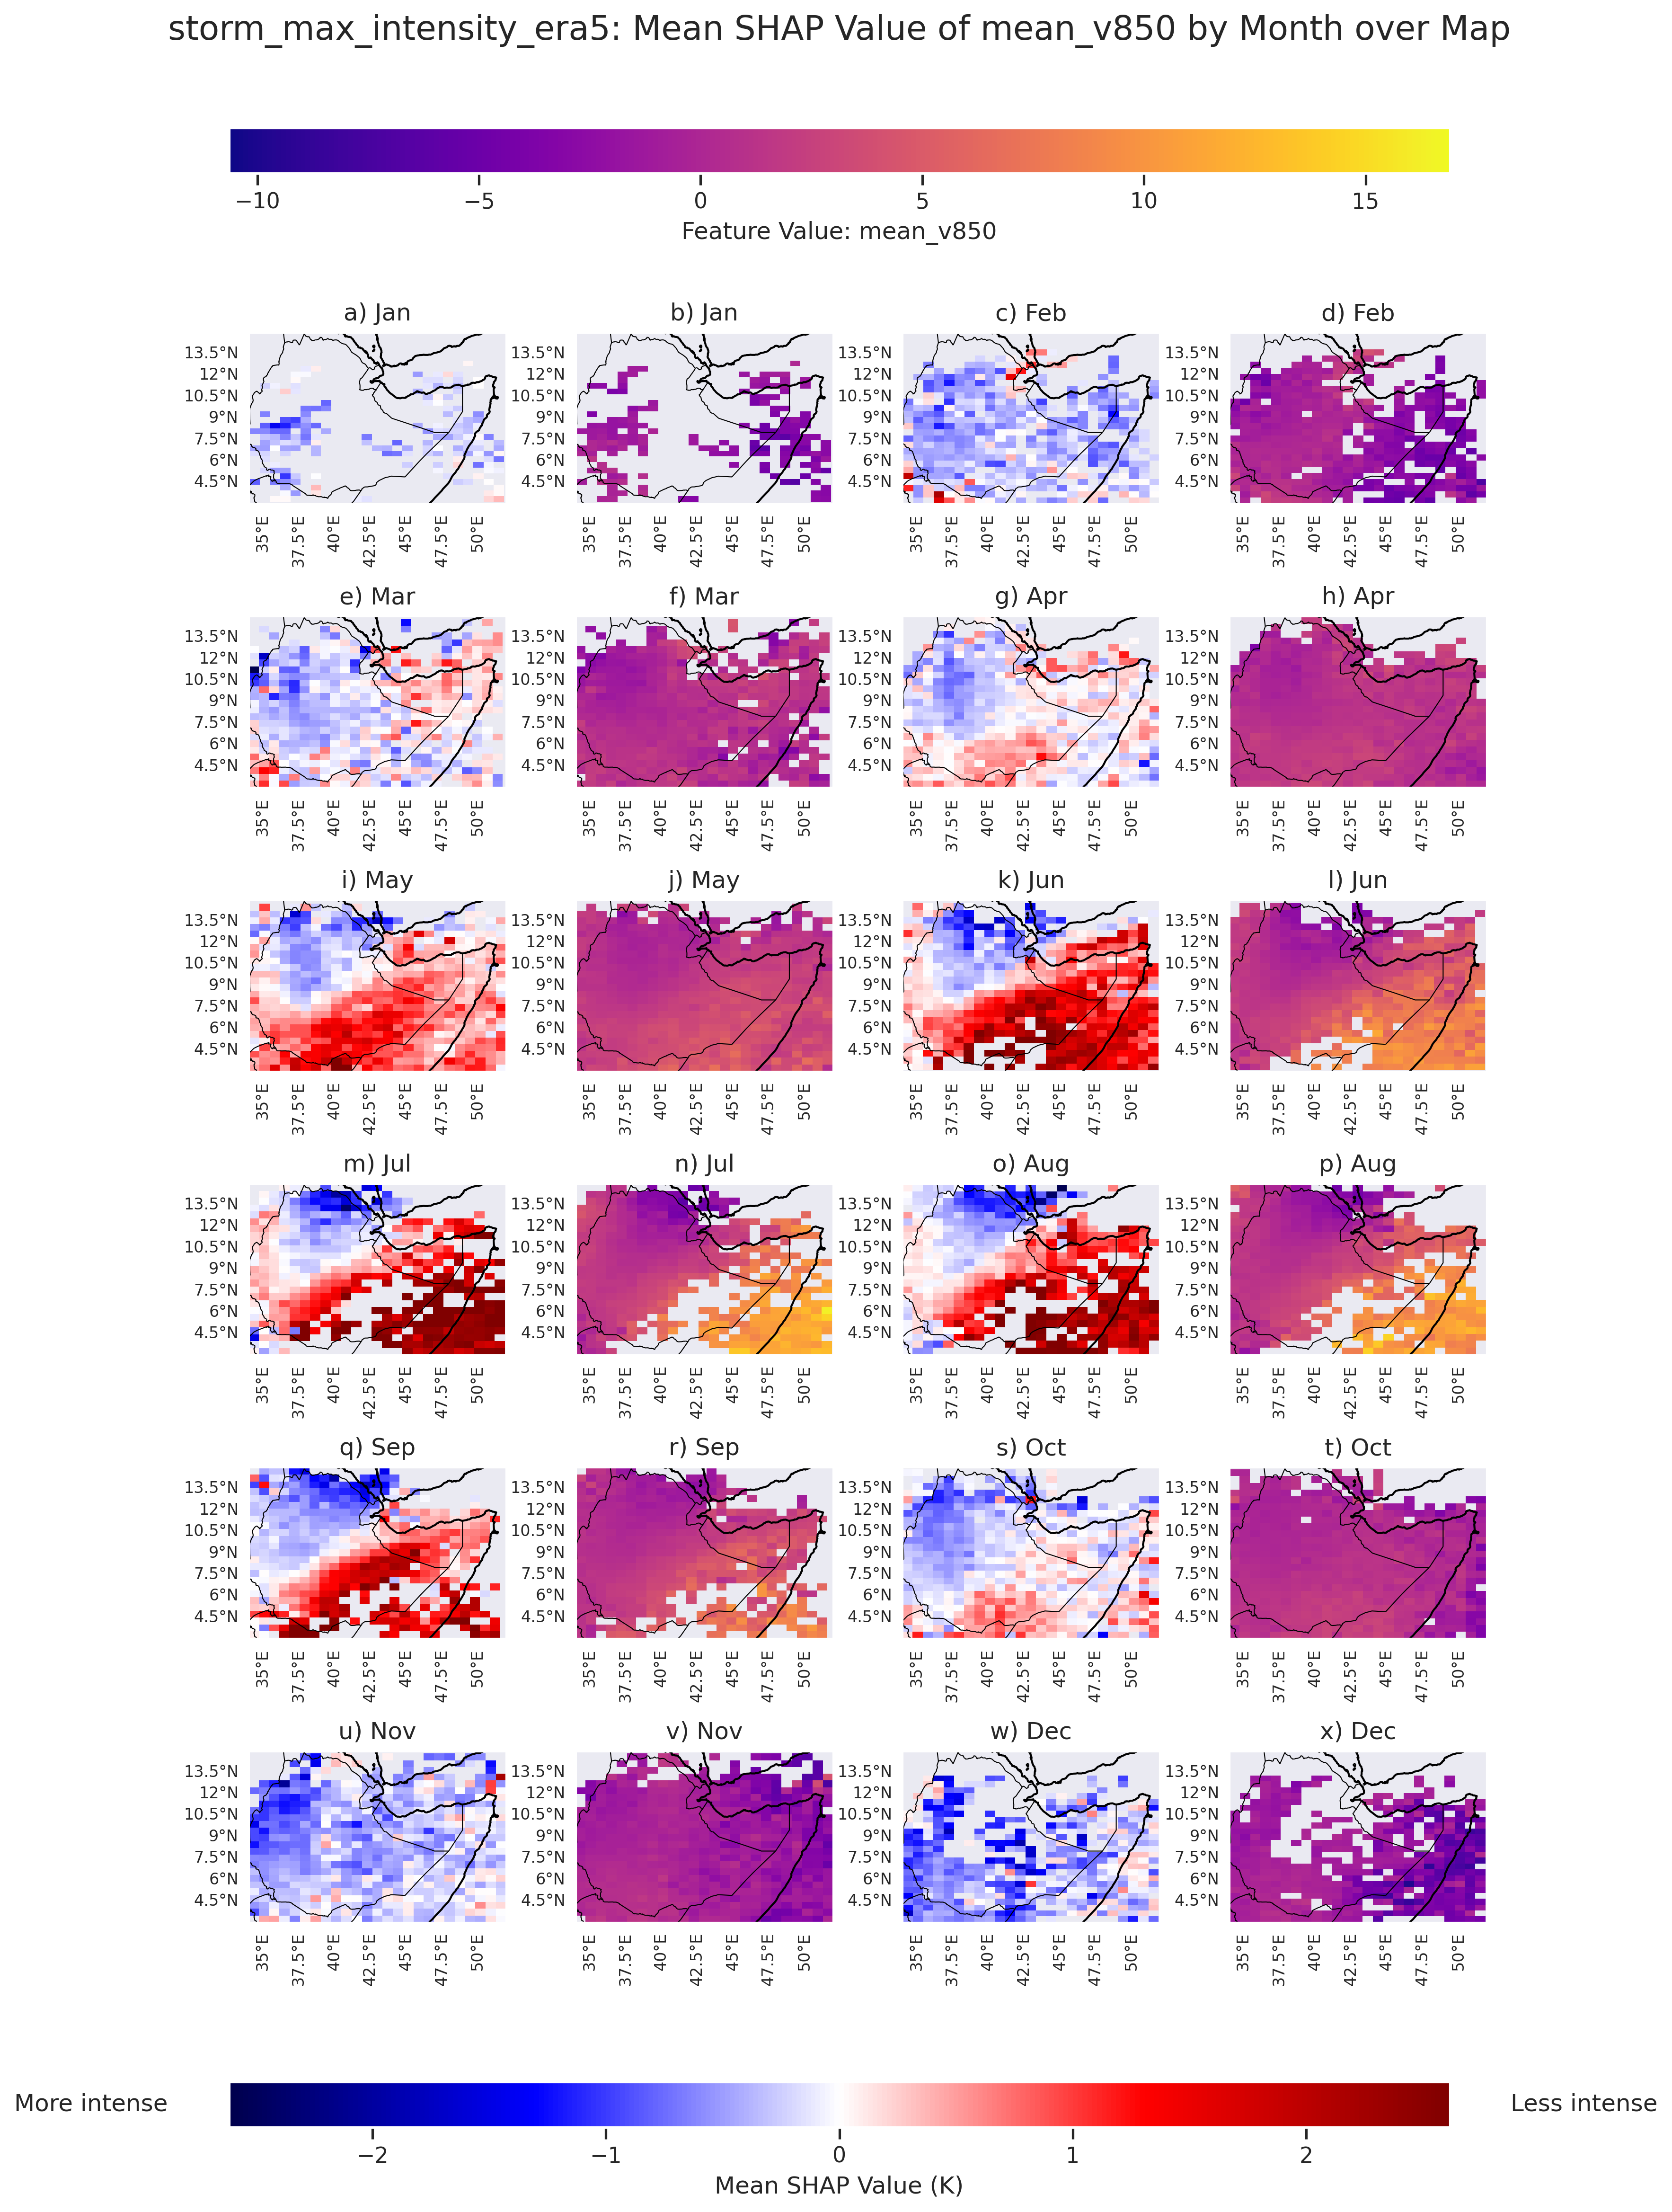
\includegraphics[width=\textwidth]{../figures/generated/experiments/storm_max_intensity/geographic_corr/storm_max_intensity_era5_shap_mean_v850_map_by_month.png}
    \caption{Mean SHAP values for 850 hPa meridional wind over East Africa by month for storm max intensity prediction using ERA5 features.}
    \label{fig:storm_max_intensity_era5_shap_mean_v850_map_by_month}
\end{figure}

\subsection{Storm Direction}

Table \ref{tab:storm_direction_results} details the performance metrics for storm direction prediction across different experimental setups as specified in the methodology.

\begin{table}[ht]
\centering
\caption{Experiment results for storm direction prediction}
\label{tab:storm_direction_results}
\begin{tabular}{lccccc}
\hline
\textbf{Experiment} & \multicolumn{2}{c}{\textbf{RMSE}} & \multicolumn{2}{c}{\textbf{Target Std}} & \textbf{Actual vs. Predicted $R^2$} \\
\cline{2-5}
 & \textbf{All} & \textbf{First pts} & \textbf{All} & \textbf{First pts} &  \\
\hline
storm\_direction\_all              & 21.8881 & 36.4077 & 75.7506 & 76.8966 & 0.9192 \\
storm\_direction\_era5             & 18.2928 & 31.6709 & 75.7506 & 76.8966 & 0.9437 \\
storm\_direction\_all\_first\_points & \multicolumn{2}{c}{61.3329} & \multicolumn{2}{c}{78.7438} & 0.3937 \\
storm\_direction\_era5\_first\_points & \multicolumn{2}{c}{61.4484} & \multicolumn{2}{c}{78.7438} & 0.3912 \\
\hline
\end{tabular}
\end{table}

Again, due to the poor performance of the first points only models, further explainability analysis will focus on the all observations models.

For better context in interpreting the meaning of the \acrshort{shap} values, Figure \ref{fig:storm_cardinal_directions_distribution} shows the distribution of storm cardinal directions in the dataset. The distribution indicates that the majority of storms move in a westerly direction. Thus, generally for this experiment, positive \acrshort{shap} values can be interpreted as shifting the predicted storm direction northward, while negative values indicate a southward shift.

\begin{figure}[h]
    \centering
    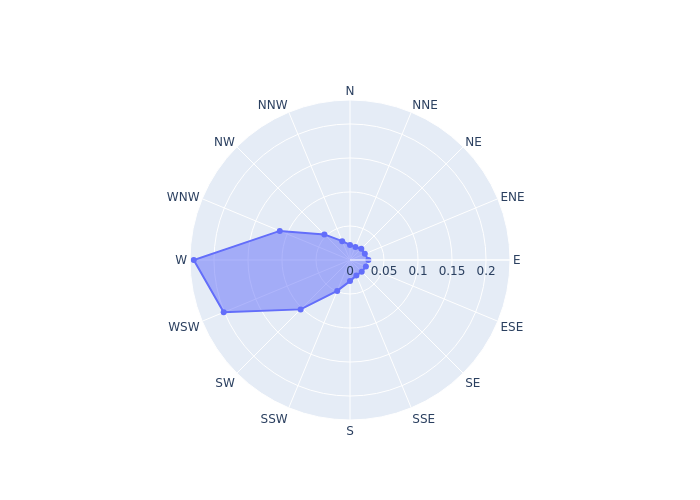
\includegraphics[width=0.8\textwidth]{../figures/generated/exploration/storm_cardinal_directions_distribution.png}
    \caption{Distribution of storm cardinal directions in the dataset.}
    \label{fig:storm_cardinal_directions_distribution}
\end{figure}



\begin{figure}[h]
    \centering
    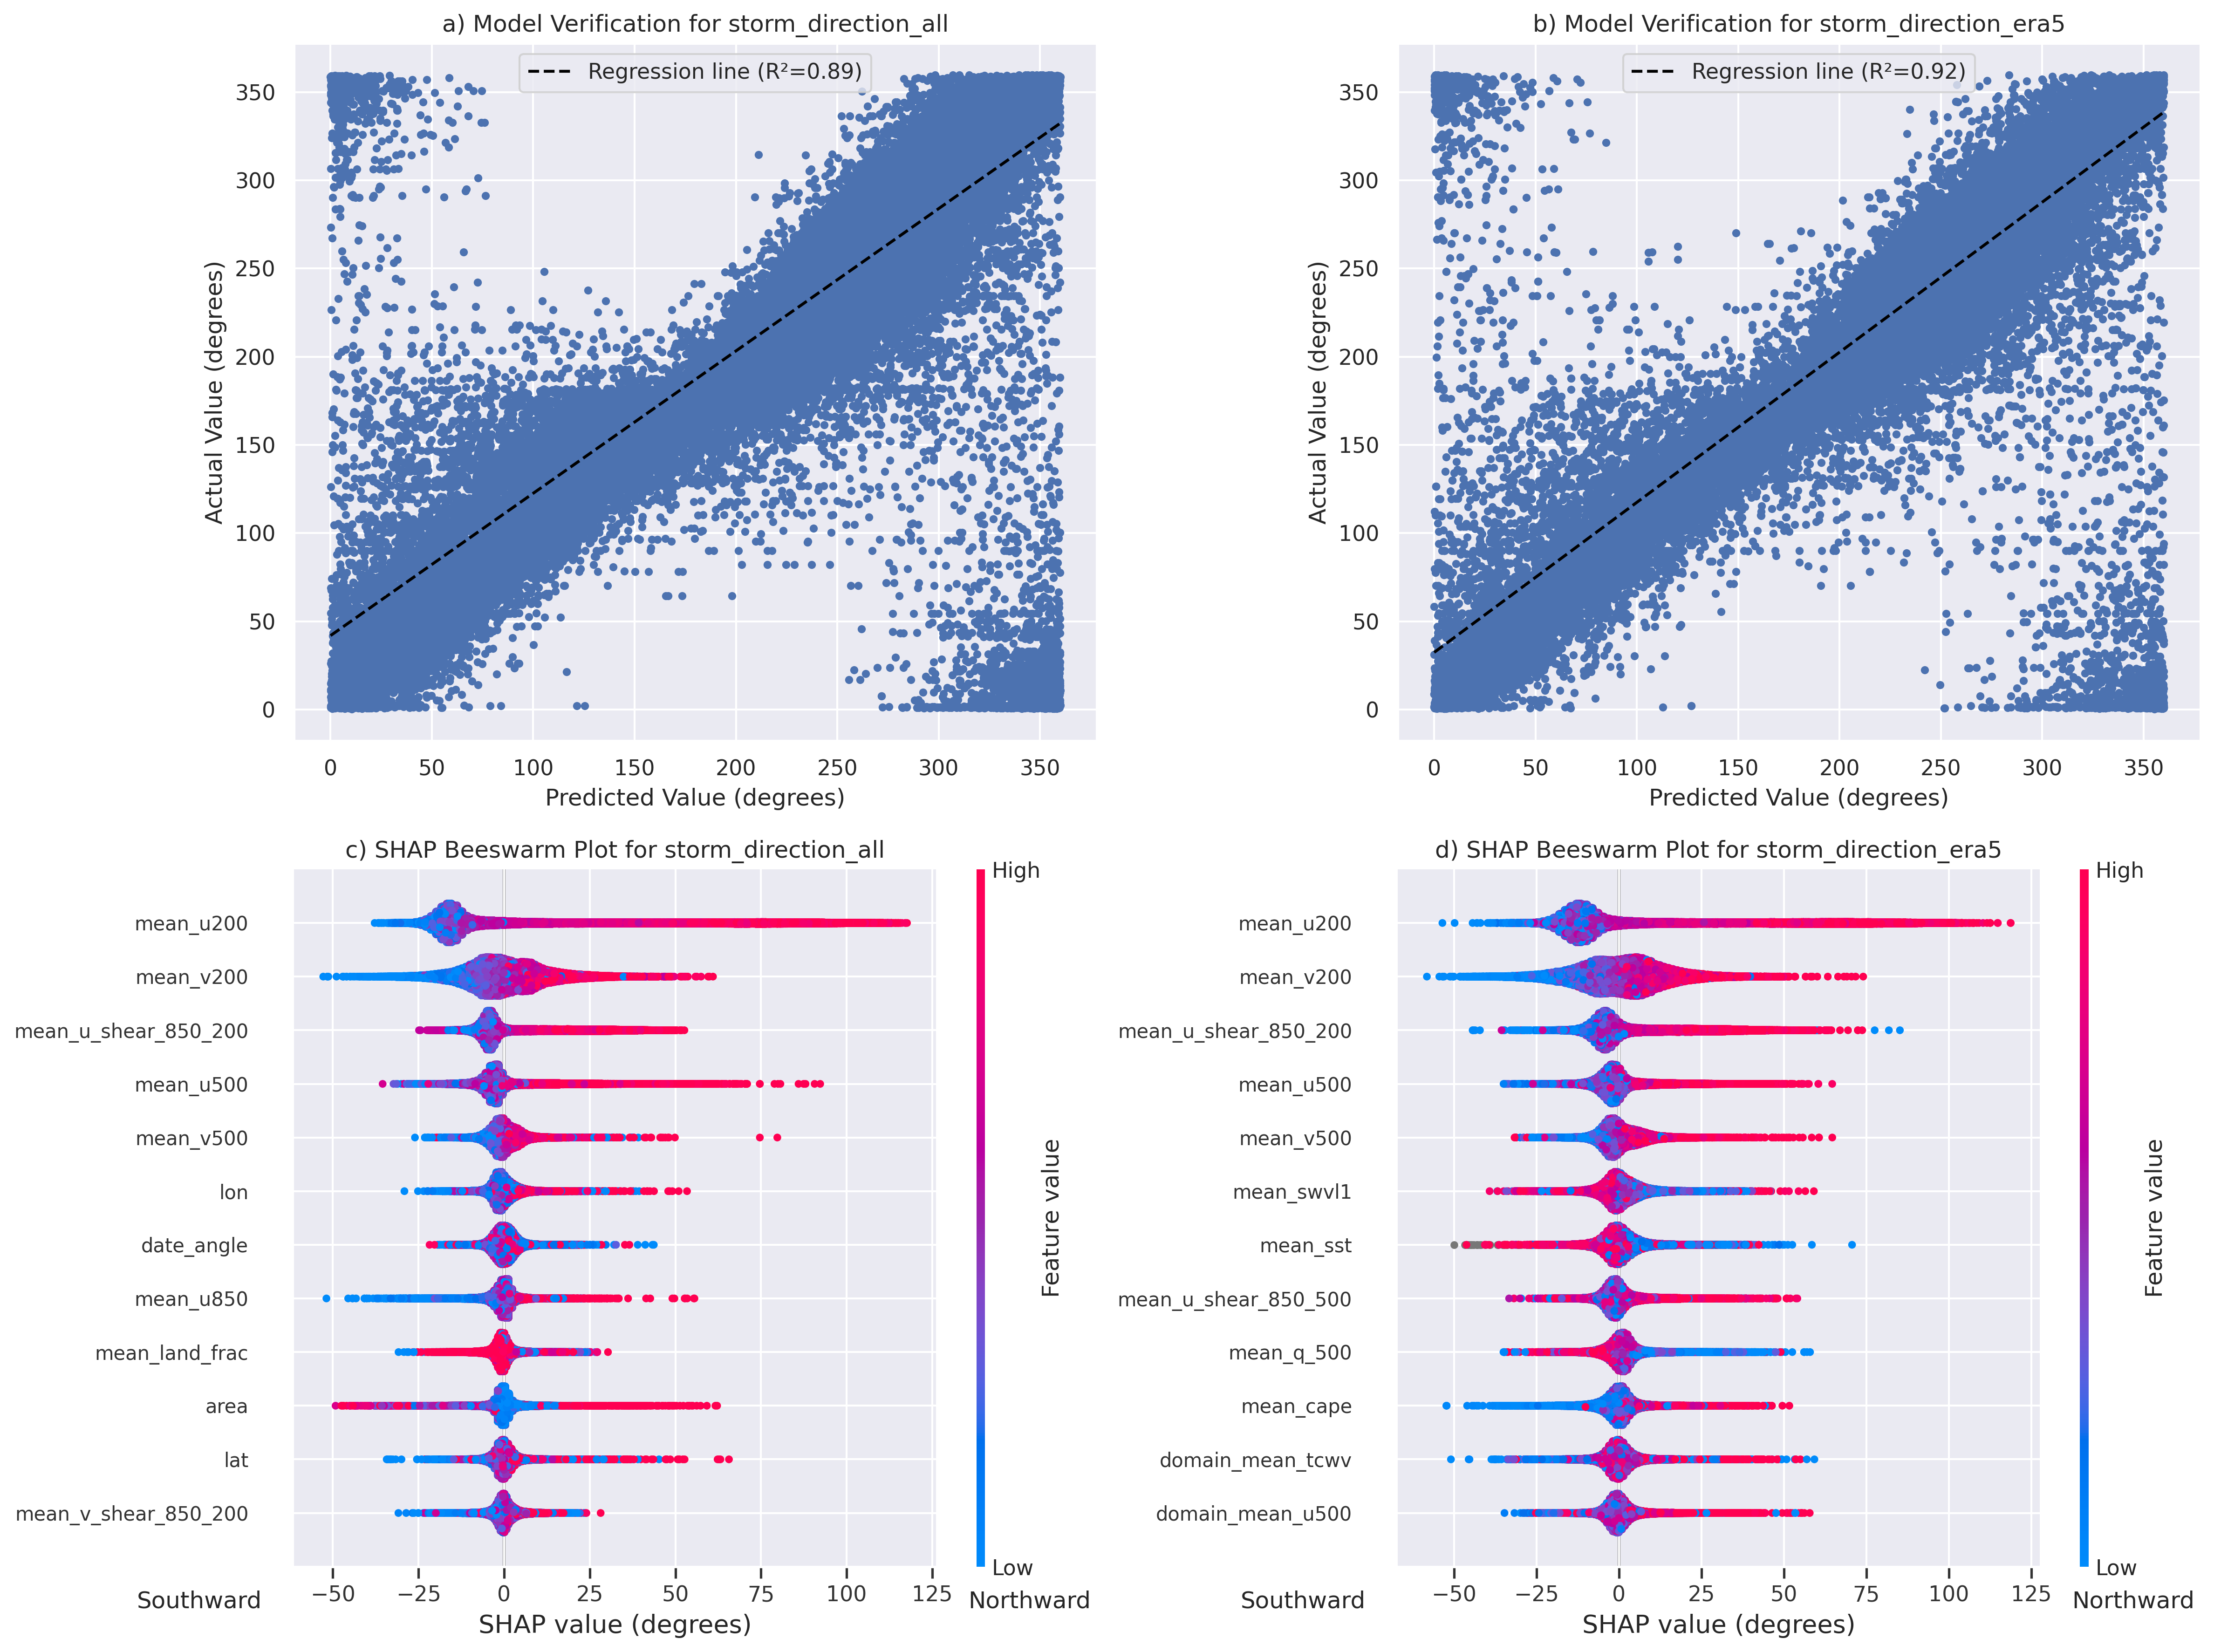
\includegraphics[width=\textwidth]{../figures/generated/experiments/storm_direction/storm_direction_summary.png}
    \caption{Comparison of performance and top features for storm direction.}
    \label{fig:storm_direction_summary}
\end{figure}






\section{Predict Immediate Characteristics at an Observation}

These experiments aim to predict the immediate characteristics of a storm based on its current observation.

\subsection{Intensification}

\begin{figure}[h]
    \centering
    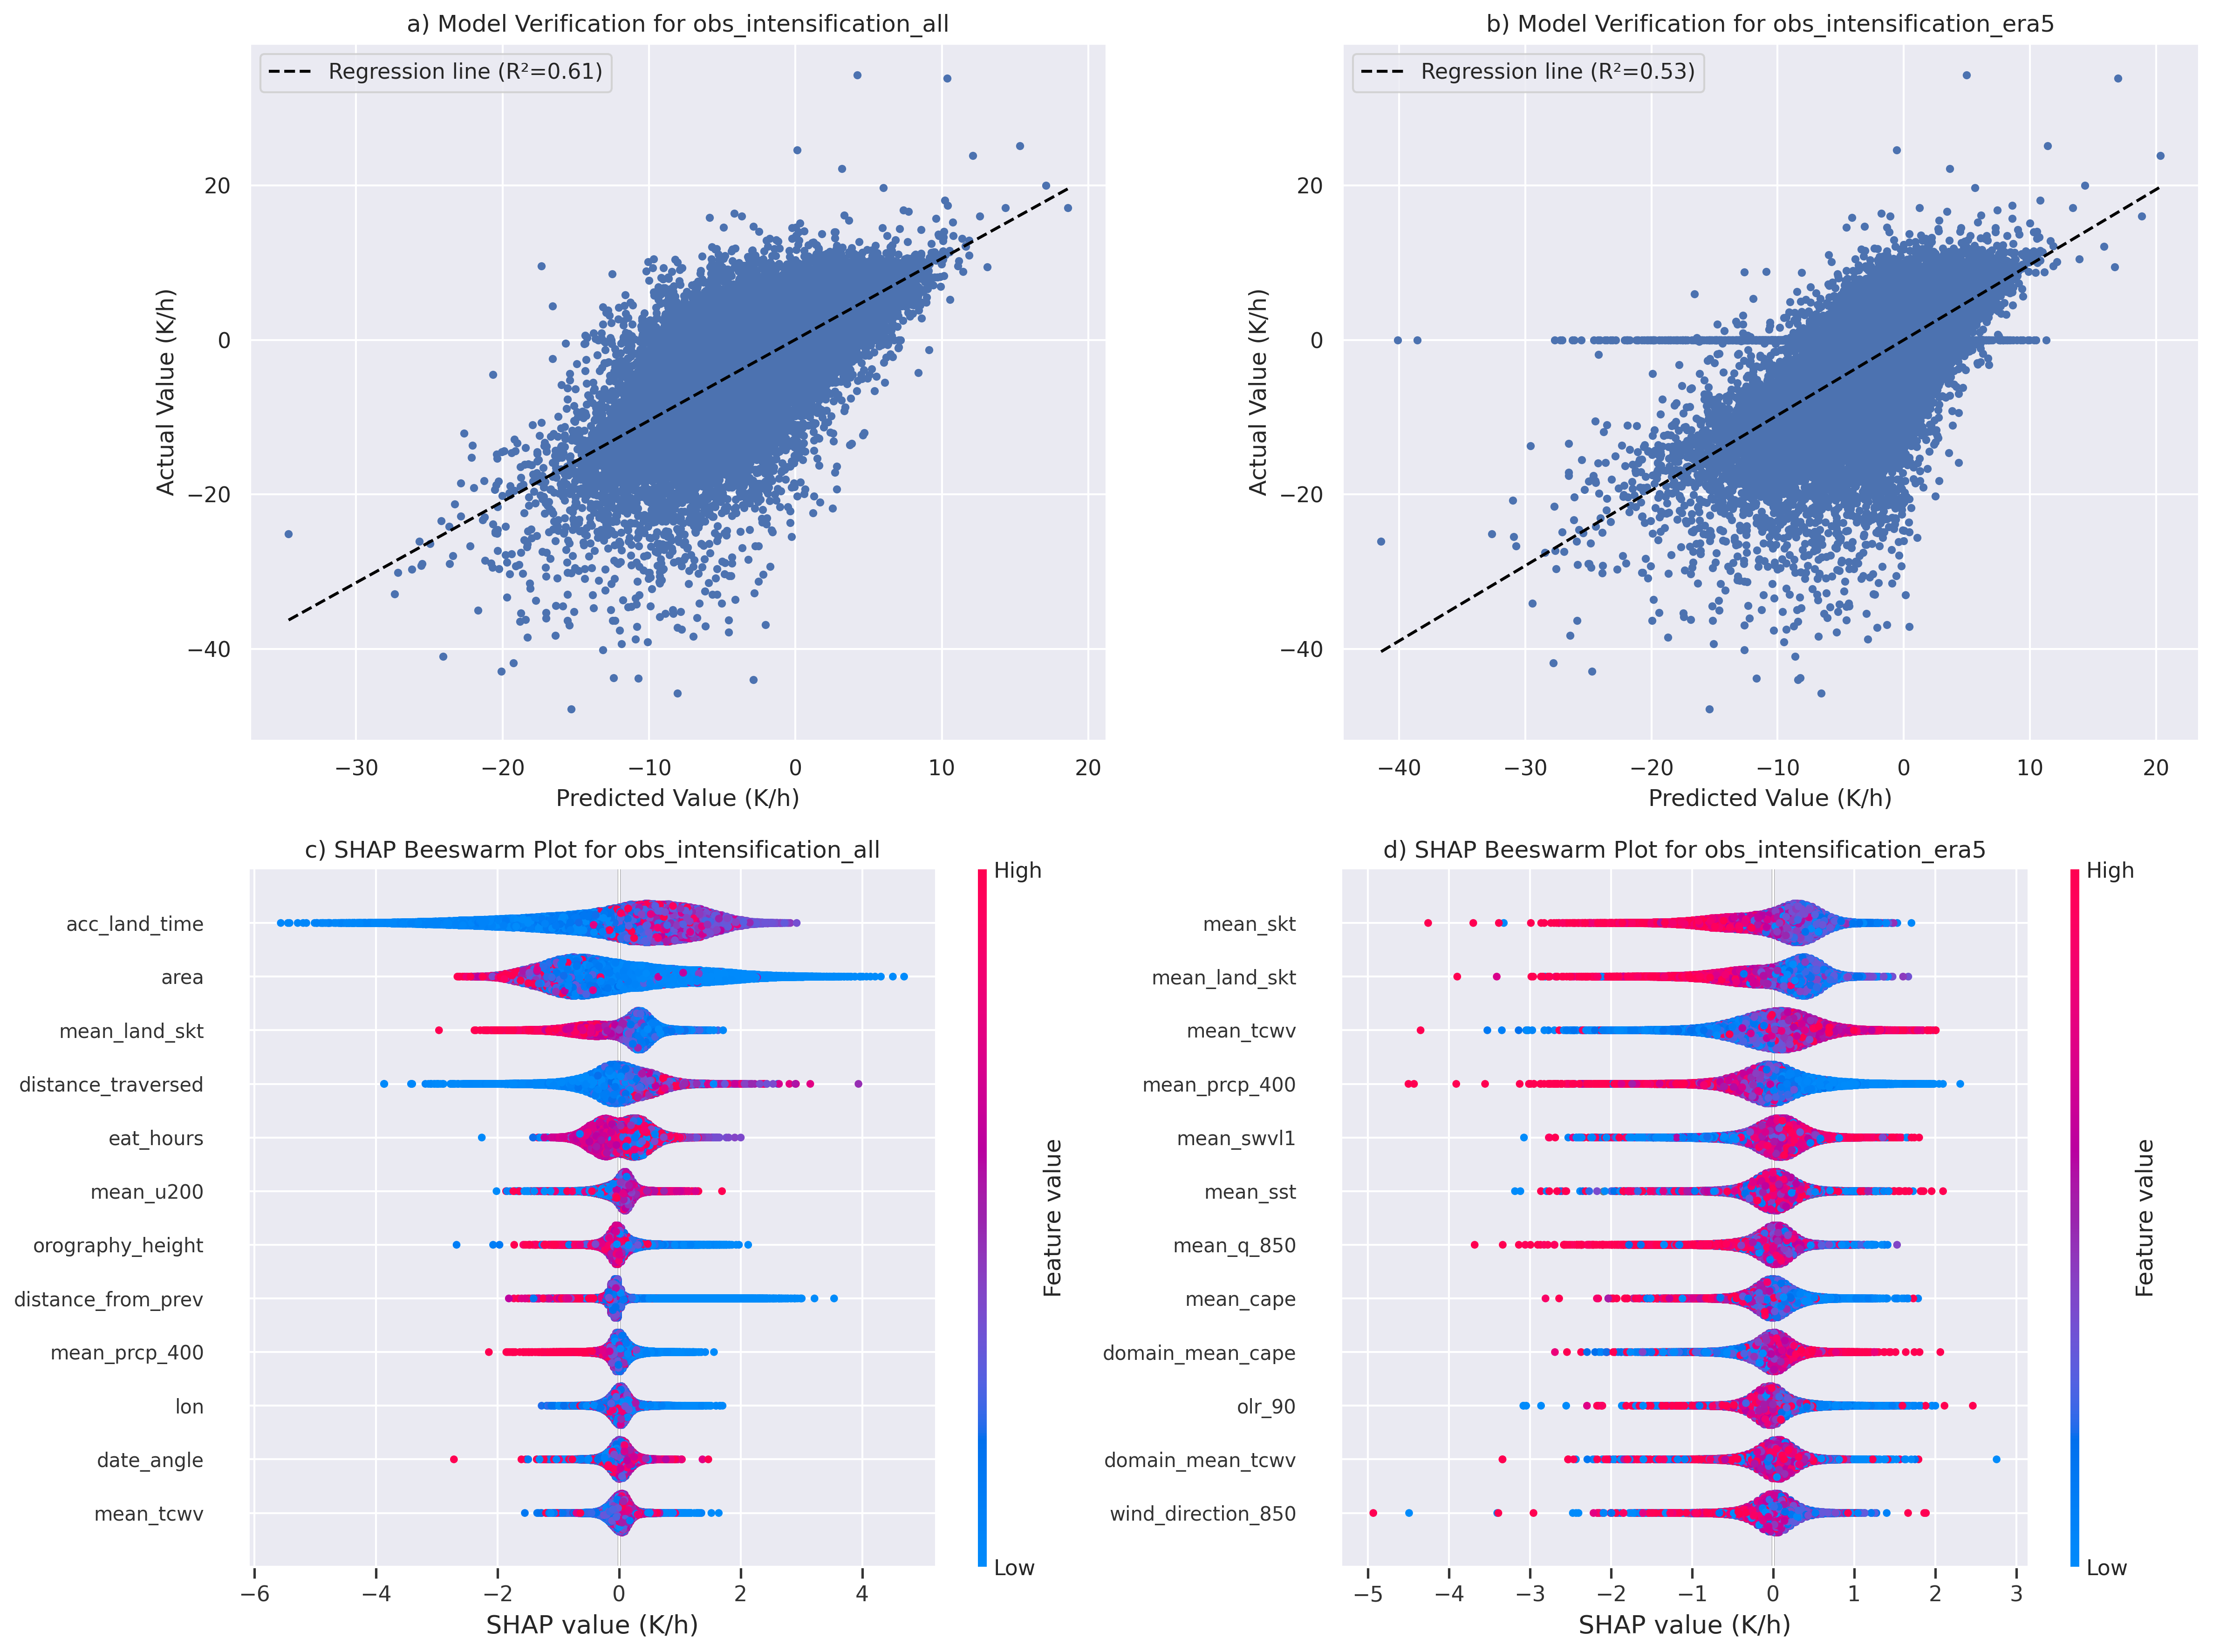
\includegraphics[width=\textwidth]{../figures/generated/experiments/obs_intensification/obs_intensification_summary.png}
    \caption{Comparison of performance and top features for intensification.}
    \label{fig:obs_intensification_summary}
\end{figure}

\subsection{Direction}

\begin{figure}[h]
    \centering
    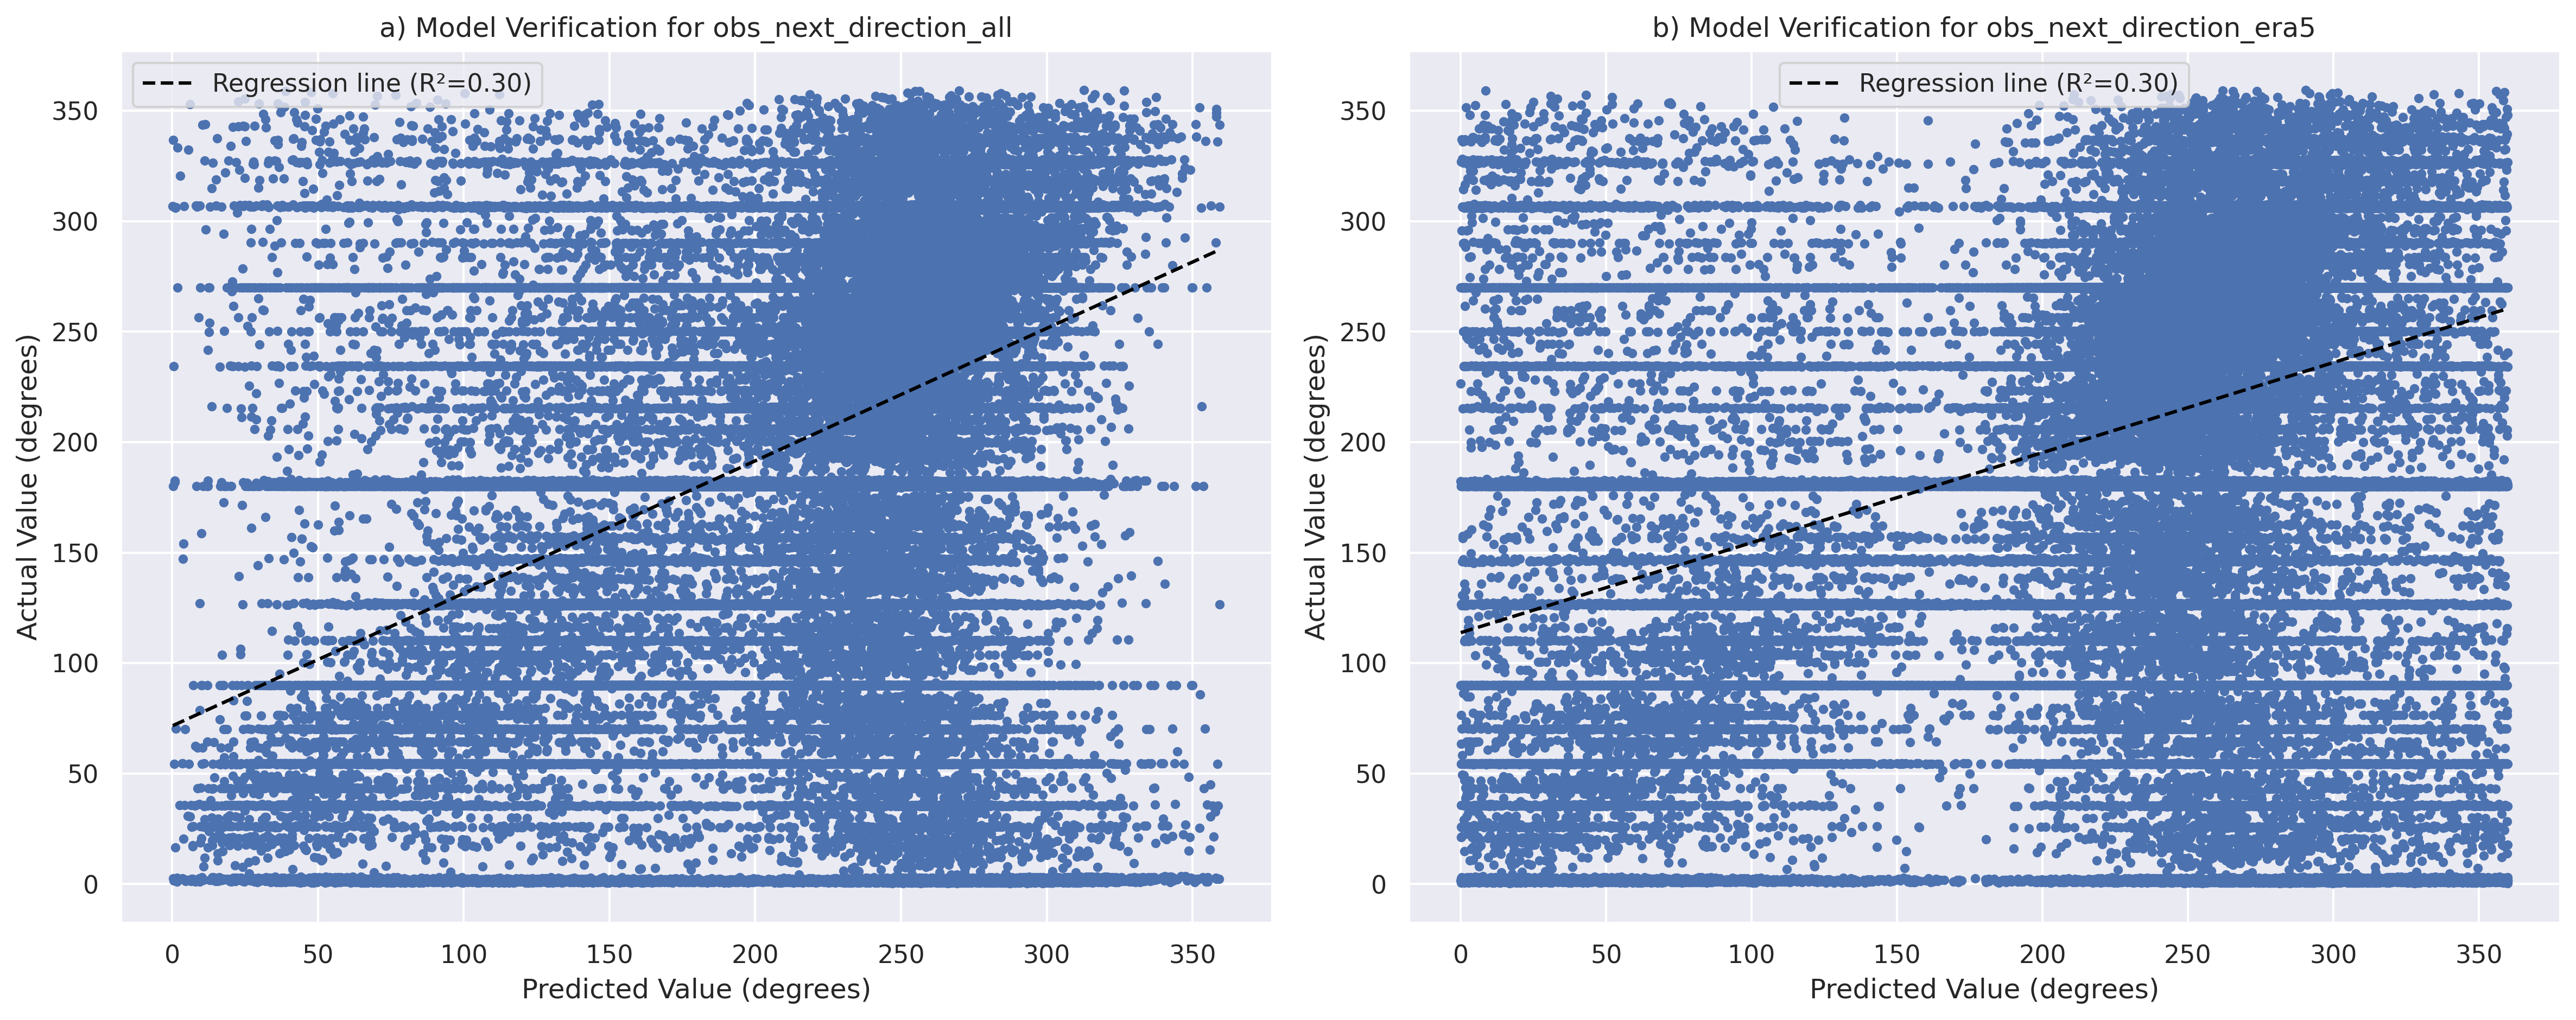
\includegraphics[width=\textwidth]{../figures/generated/experiments/obs_next_direction/obs_next_direction_summary.png}
    \caption{Comparison of performance and top features for direction.}
    \label{fig:obs_direction_summary}
\end{figure}

\subsection{Distance}

\begin{figure}[h]
    \centering
    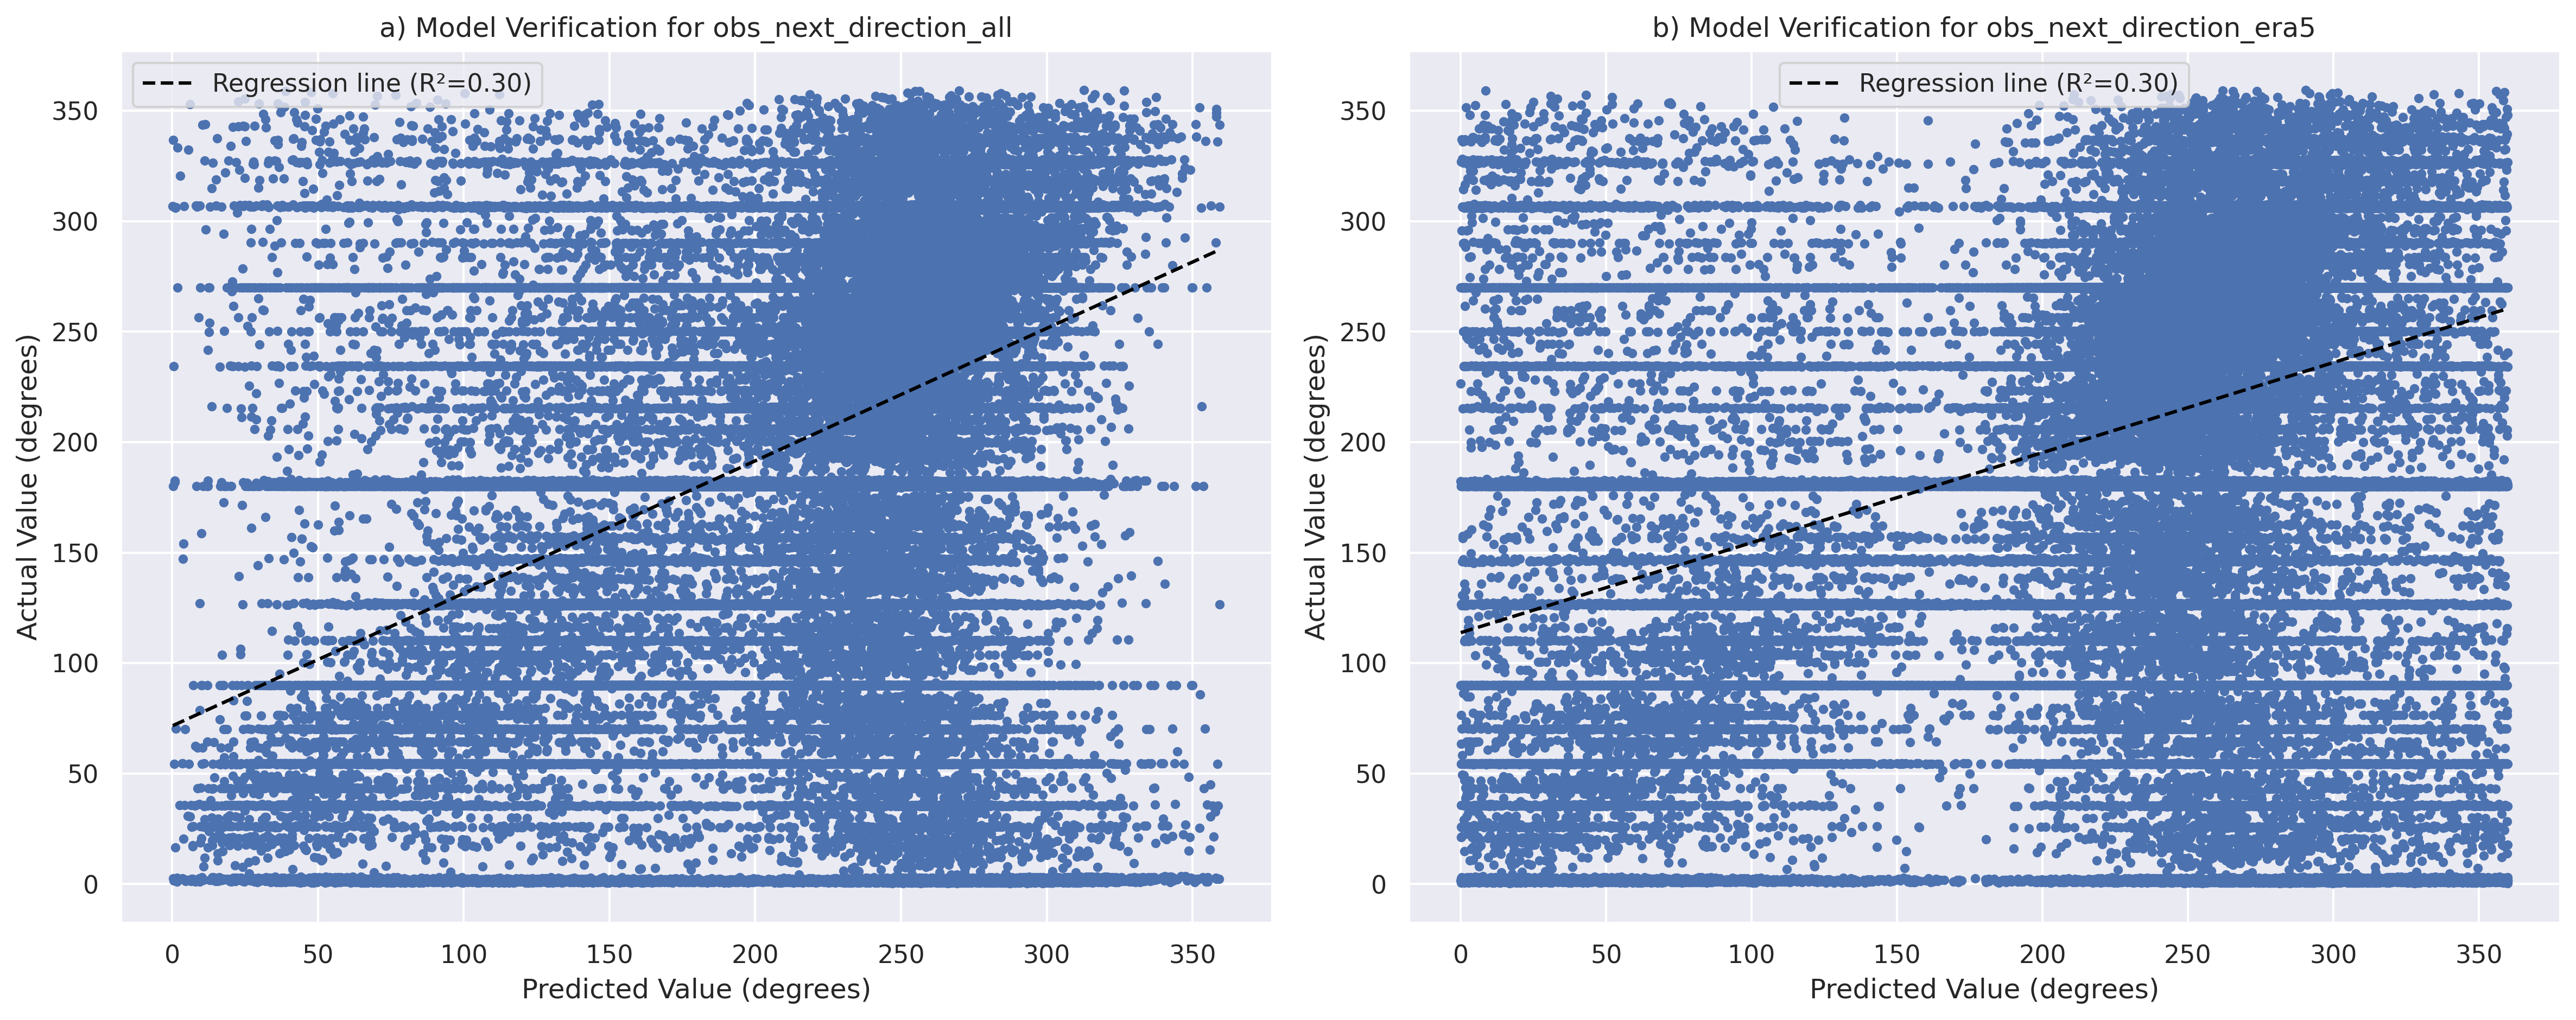
\includegraphics[width=\textwidth]{../figures/generated/experiments/obs_next_direction/obs_next_direction_summary.png}
    \caption{Comparison of performance and top features for distance.}
    \label{fig:obs_distance_summary}
\end{figure}

\subsection{Precipitation}

\begin{figure}[h]
    \centering
    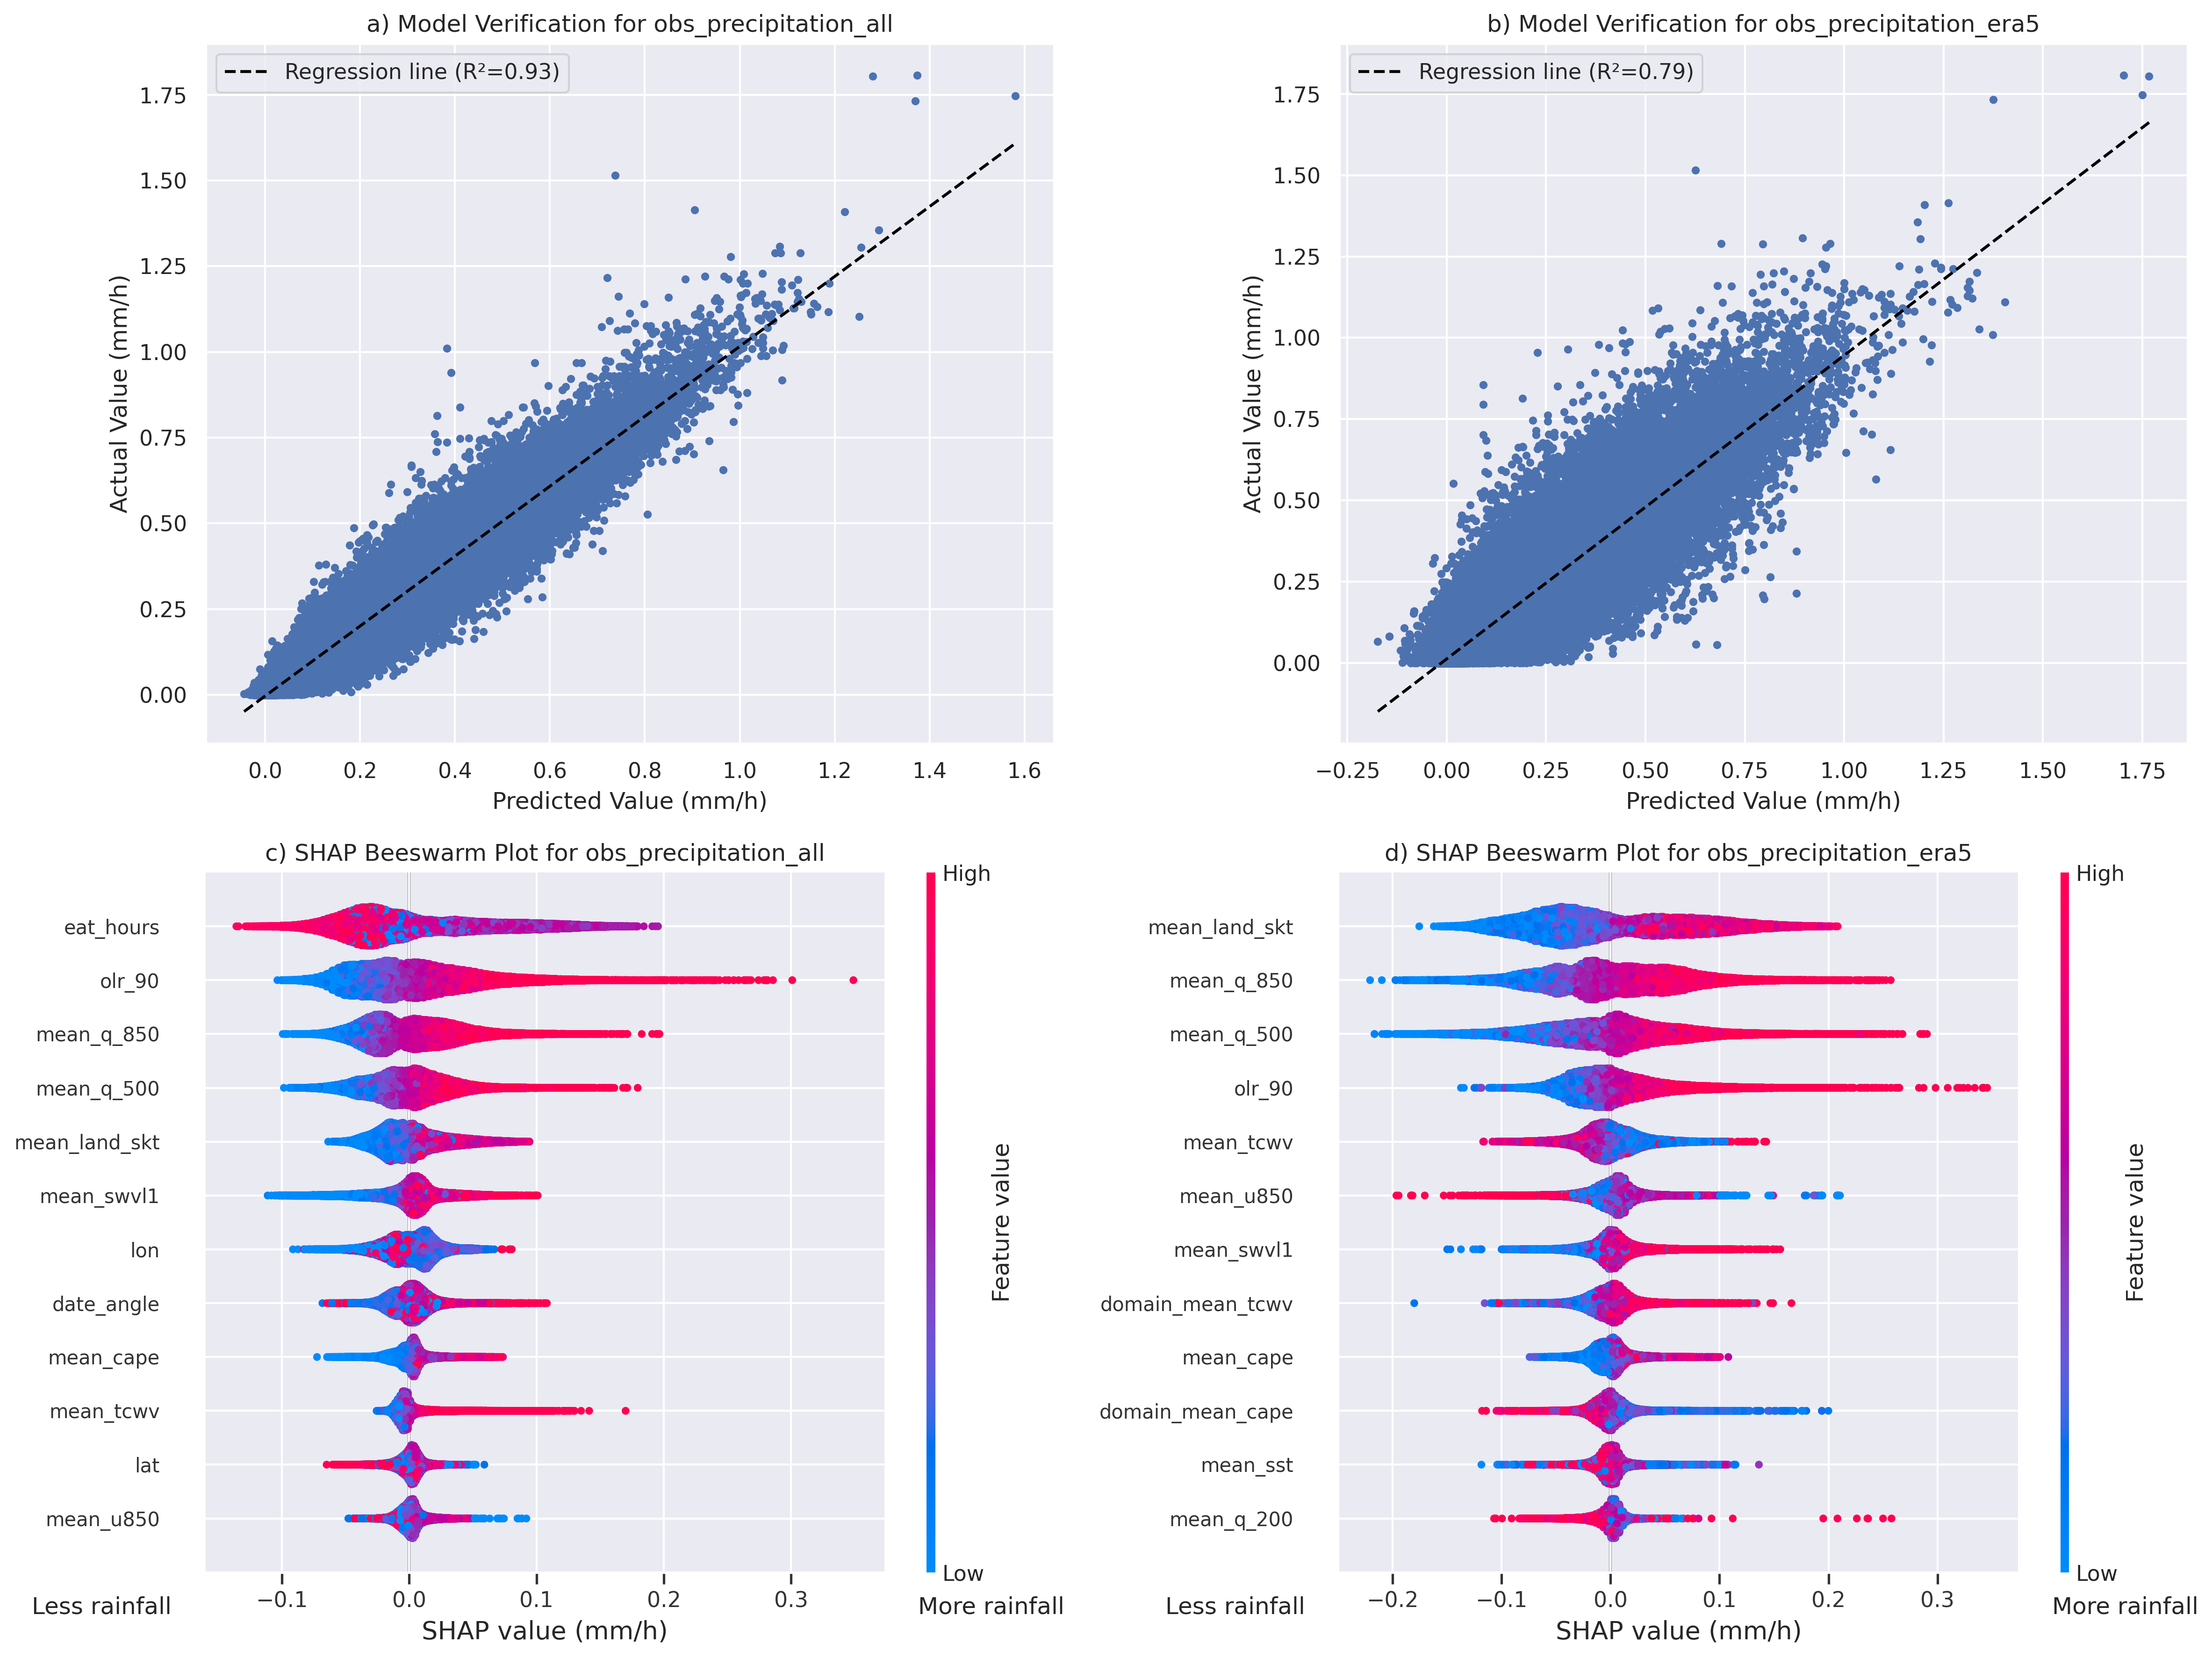
\includegraphics[width=\textwidth]{../figures/generated/experiments/obs_precipitation/obs_precipitation_summary.png}
    \caption{Comparison of performance and top features for precipitation.}
    \label{fig:obs_precipitation_summary}
\end{figure}